
\section*{Linear Classifiers}

    If you wanted to break up your data into two parts ($+1$ and $-1$), how might you do it? Let's explore that question.
    
    \subsection*{1-D Linear Classifiers}
    
        As usual, we'll start with the \textbf{simplest} case we can think of: 1-D. So, we only have one variable $x_1$ to \textbf{classify} with.
        
        The simplest version might be to just \textbf{split} our space in \textbf{half}: those above or below a certain \textbf{value}. This is our parameter, $C$.
        
        \begin{equation}
            x_1 > C \qquad \text{or} \qquad x_1 - C > 0
        \end{equation}
        
        \miniex For the below data (where green gives positive and red gives positive), could classify positive as $x_1>3$.
        
        \begin{figure}[H]
            \centering
            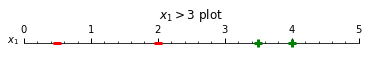
\includegraphics[width=70mm,scale=0.4]{images/classification_images/x1_1d_plot_points.png}

            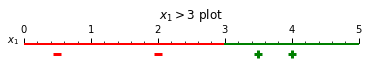
\includegraphics[width=70mm,scale=0.4]{images/classification_images/x1_1d_plot.png}
            
            \caption*{We plot everything above $x=3$ as \textbf{positive}, and \textbf{negative} otherwise.}
        \end{figure}
        
        We could also call it $\theta_0$, in the spirit of our $\theta$ notation for parameters.
        
        \begin{equation}
            x_1 + \theta_0 > 0
        \end{equation}
    
    \subsection*{1-D classifiers in 2-D}
        
        Let's add a variable and see how our classifier looks on a 2-D plot.
            \note{We'll omit the data points for now.}
        
        \begin{figure}[H]
                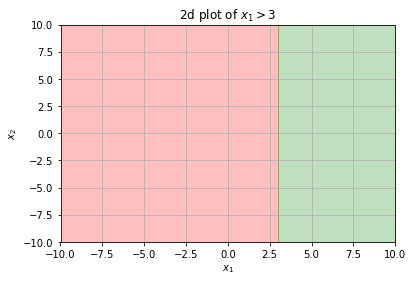
\includegraphics[width=70mm,scale=0.5]{images/classification_images/x1_2d_plot.png}
                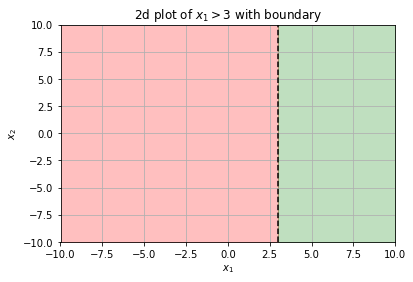
\includegraphics[width=70mm,scale=0.5]{images/classification_images/x1_2d_plot_boundary.png}
                
                \caption*{On the right, we've drawn the \textbf{dividing} line between our two regions.}
        \end{figure}
        
        Interesting - the \textbf{boundary} between positive and negative is defined by a \textbf{vertical line}.
        
        Or, almost. Compare $x_1>3$ and $x_1<3$:
        
        \begin{figure}[H]
                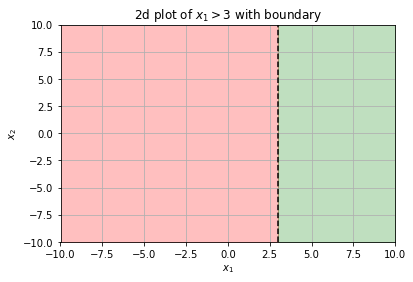
\includegraphics[width=70mm,scale=0.5]{images/classification_images/x1_2d_plot_boundary.png}
                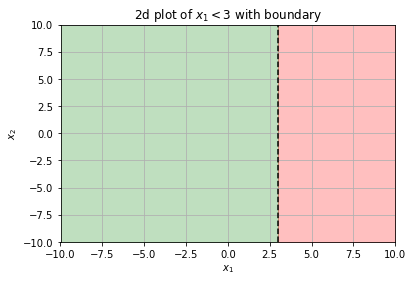
\includegraphics[width=70mm,scale=0.5]{images/classification_images/x1_2d_plot_boundary_reversed.png}
                
                \caption*{These two plots have the same line, but have their sides flipped.}
        \end{figure}
        
        So, we have a \textbf{line} that gives us the boundary, but we \textbf{also} need to include information about which way is the \textbf{positive} direction.
        
        What tool best represents \textbf{direction}? We could use angles, but we haven't used that much so far. Instead, let's use a \textbf{vector} to \textbf{point} in the right direction.
        
        \begin{figure}[H]
                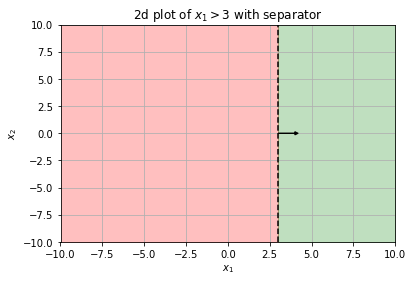
\includegraphics[width=70mm,scale=0.5]{images/classification_images/x1_2d_plot_separator.png}
                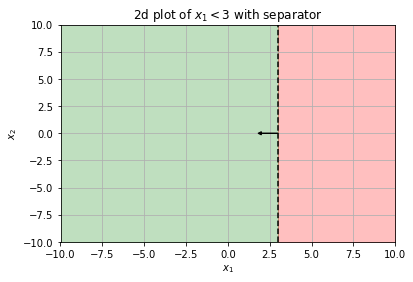
\includegraphics[width=70mm,scale=0.5]{images/classification_images/x1_2d_plot_separator_reversed.png}
                
                \caption*{Now, it's clear which plot is which, just using our \textbf{line} and \textbf{vector}!}
        \end{figure}
        
        The object that represents our classification is called a \textbf{separator}!
            \note{Since our variables are $x_1$ and $x_2$, this is a separator in \textbf{input space}.}\\
            
        \begin{definition}
            A \vocab{separator} defines how we \gren{separate} two different classes with our \purp{hypothesis}.
            
            It includes
            
            \begin{itemize}
                \item The \vocab{boundary}: the \gren{surface} where we \purp{switch} from one \purp{class} to another.
                \item The \vocab{orientation}: a \gren{description} of which \purp{side} of the boundary is assigned to \purp{which class}.
            \end{itemize}
        \end{definition}
        
        \note{We call it "orientation" because you could imagine "flipping over" the space, so the positive and negative regions are swapped.}
        
        For example, let's take our specific separator from above.\\
        
        \begin{concept}
            We can define our \vocab{1-D separator} using
            
            \begin{itemize}
                \item The \vocab{boundary} between the \gren{positive} and \redd{negative} regions: in 2-D input space, this looks like a vertical or horizontal \purp{line}.
                
                \item A \vocab{vector} pointing towards whichever side is given a \gren{${+1}$ value}.
            \end{itemize}
        \end{concept}
    
    \subsection*{A second 1-D separator, and our problem}
        
        What if we use $x_2$ to \textbf{separate} our data?
        
        \begin{figure}[H]
                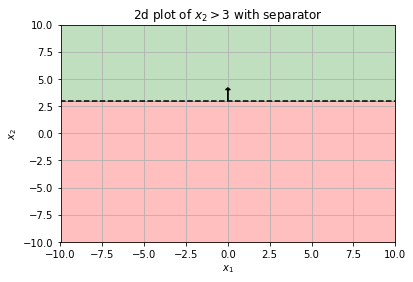
\includegraphics[width=70mm,scale=0.5]{images/classification_images/x2_2d_plot_separator.png}
                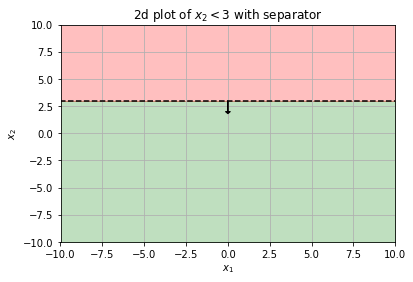
\includegraphics[width=70mm,scale=0.5]{images/classification_images/x2_2d_plot_separator_reversed.png}
                
                \caption*{Instead of having a vertical separator, we have a \textbf{horizontal} one.}
        \end{figure}
        
        We get the same sort of plot along the \textbf{other axis}!
        
        So, this is cool so far, but it's not a very \textbf{powerful} model: we can only handle a situation where the data is evenly divided by \textbf{one axis}.
        
        And if that's the case, what's the point of our \textbf{other} variable?
        
        \begin{figure}[H]
            \centering
                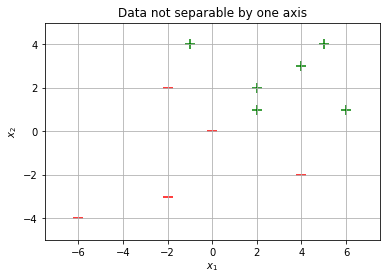
\includegraphics[width=70mm,scale=0.5]{images/classification_images/data_not_1d_separable.png}
                
                \caption*{There's no vertical or horizontal line we can use to split this space!}
        \end{figure}
        
    \subsection*{The 2-D Separator: What vector do we use?}
    
        Just looking at our example, we might wonder, "well, if we can use \textbf{vertical} lines or \textbf{horizontal} lines, can't we just use a line in \textbf{another} orientation?
        
        It turns out, we \textbf{can}!
        
        \begin{figure}[H]
            \centering
                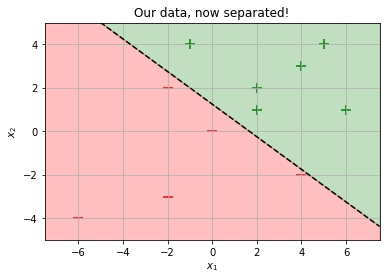
\includegraphics[width=70mm,scale=0.5]{images/classification_images/data_2d_separable.png}
                
                \caption*{If allow lines at an angle, we can classify all of our data correctly!}
        \end{figure}
        
        So, we've got our \textbf{boundary}. But we still need a vector to tell us which side is \textbf{positive}. But there are \textbf{many} possible vectors we could choose:
        
        \begin{figure}[H]
            \centering
                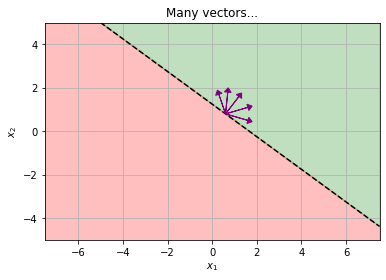
\includegraphics[width=70mm,scale=0.5]{images/classification_images/many_vectors_for_a_plane.png}
                
                \caption*{All of these vectors point towards the \textbf{correct} side of the plane. Is there a \textbf{best} one to use?}
        \end{figure}
        
        Above, we used the vector that was \textbf{vertical} or \textbf{horizontal}. This makes sense: if we're doing $x_1>3$, it seems reasonable to have the arrow \textbf{point} in the positive-$x_1$ direction.
        
        But this vector also happened to be \textbf{perpendicular} to our \textbf{line}: this is the line's \textbf{normal vector}, $\hat{n}$. This vector has a couple nice properties:
        
        \begin{itemize}
            \item It is \textbf{unique}: in 2-D, there is only 1 \textbf{normal} direction.
                \note{The opposite side is just $-\hat{n}$.}
                
            \item It points directly \textbf{away} from the plane.
            
            \item If our plane is at the \textbf{origin}, any point with a \textbf{positive} $\hat{n}$ component is on the \textbf{positive} side.
                \note{This will be important later!}
        \end{itemize}
        
        So, we have a \textbf{unique} vector that tells us which side is \textbf{positive}. Let's go with that!\\
        
        \begin{concept}
            Every \gren{line} in 2-D has a \vocab{unique normal vector} that can be used to \purp{define} the \gren{angle/direction} of the line.
            
            The \purp{direction} the vector is "facing" is also called the \vocab{orientation}.
        \end{concept}
        
        Our normal vector for the above separator:
        
        \begin{figure}[H]

                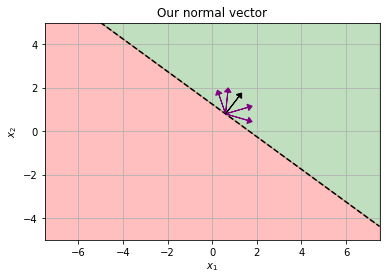
\includegraphics[width=70mm,scale=0.5]{images/classification_images/normal_vector_among_others.png}
                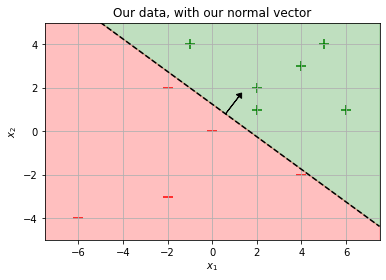
\includegraphics[width=70mm,scale=0.5]{images/classification_images/data_2d_separable_normal vector.png}
                
                \caption*{We can define our plane using the \textbf{normal} vector!}
        \end{figure}
        
        It's clear that this vector in some way is a \textbf{parameter}: if we change this vector, we get a different \textbf{orientation}, and a different \textbf{classifier}. 
        
        We have \textbf{represented} parameters in the past using $\theta$. We need \textbf{two} different $\theta_k$: one for the $x_1$ component, another for the $x_2$ component.
        
        So, we'll use that.\\
        
        \begin{notation}
            The vector $\theta$ represents the \vocab{normal vector} to our line in 2D.
            
            \begin{equation*}
                \hat{n} = \theta =
                \begin{bmatrix}
                        \theta_1 \\
                        \theta_2
                \end{bmatrix}
            \end{equation*}
        \end{notation}
        
        We add this to our diagram:
        
        \begin{figure}[H]
                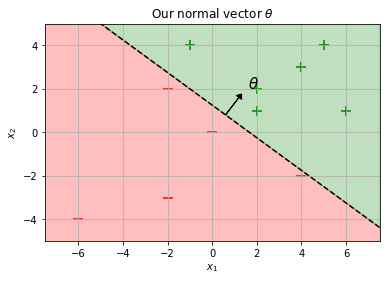
\includegraphics[width=70mm,scale=0.5]{images/classification_images/normal_vector_theta.png}
                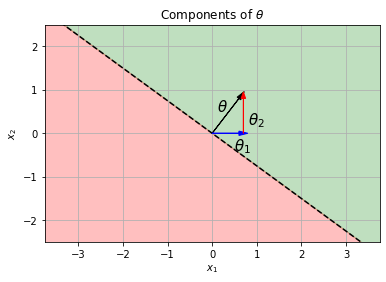
\includegraphics[width=70mm,scale=0.5]{images/classification_images/theta_components.png}
                
                \caption*{$\theta$ is our normal vector!}
        \end{figure}
        
        Nice work so far. The next question is: how do we describe this separator \textbf{mathematically}?
        
    \subsection*{2D Separator - Matching components}
    
        As always, we'll \textbf{simplify} the problem to make it more manageable: for now, we'll assume our \textbf{separator} is centered at the \textbf{origin}.
        
        \begin{figure}[H]
            \centering
                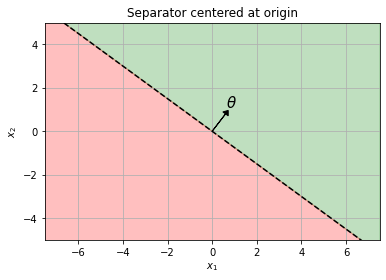
\includegraphics[width=70mm,scale=0.5]{images/classification_images/separator_centered_at_origin.png}
        \end{figure}
        
        So, we have our vector, $\hat{n}$. As we mentioned above, anything on the \textbf{same} side as $\hat{n}$ is \textbf{positive}, and anything on the \textbf{opposite} side is \textbf{negative}.
            \note{For a line on the origin, "On the same side of the line" can be interpreted as "has a positive $\hat{n}$ component". We'll find that component next.}\\
            
        \begin{figure}[H]
                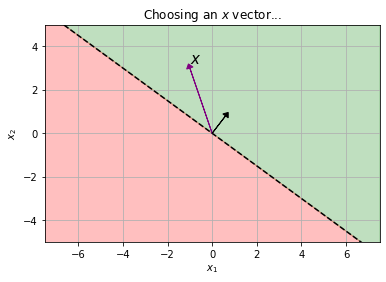
\includegraphics[width=70mm,scale=0.5]{images/classification_images/chose_a_vector.png}
                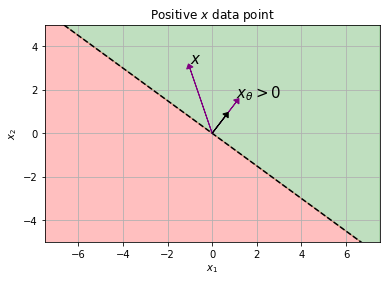
\includegraphics[width=70mm,scale=0.5]{images/classification_images/positive_v_vector.png}
                
                \caption*{This vector has a \textbf{positive} component in the $\theta$ direction.}
        \end{figure}
        
        \begin{figure}[H]
            \centering
                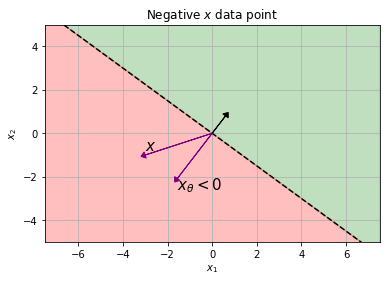
\includegraphics[width=70mm,scale=0.5]{images/classification_images/negative_v_vector.png}
                
                \caption*{This vector has a \textbf{negative} component in the $\theta$ direction.}
        \end{figure}
            
        How do we represent "on the same side" mathematically? How do we \textbf{find} whether the component is \textbf{positive} or \textbf{negative}? We use the \textbf{dot product}.\\
        
    \subsection*{The Dot Product (Review)}
    
        How to calculate the dot product should be familiar to you, but we'll talk about some \textbf{intuition} that you may not be exposed to.\\
        
        \begin{concept}
            You can use the \vocab{dot product} between unit vectors to measure their "\purp{similarity}": if two vectors are more \gren{similar}, they have a \gren{larger} dot product.
            
            In the most clear cases, take unit vectors $\hat{a}$ and $\hat{b}$:
            
            \begin{itemize} 
                \item If they are in the \vocab{exact same} direction, $\hat{a} \cdot \hat{b} = 1$
                
                \item If they are in the \vocab{exact opposite} direction, $\hat{a} \cdot \hat{b} = -1$
                
                \item If they are \vocab{perpendicular} to each other, $\hat{a} \cdot \hat{b} = 0$
            \end{itemize}
        \end{concept}
        
            \note{Remember, \textbf{unit vectors} have a length of 1.}
        
        What about non-unit vectors?
        
        These unit vectors are then scaled up by the \textbf{magnitude} of each of our vectors. Because magnitudes are \textbf{always positive}, the dot product sign doesn't change.\\
        
        \begin{concept}
            You can use the \vocab{dot product} between non-unit vectors to measure their "similarity" \purp{scaled by their magnitude}. 
            
            If two vectors are more \gren{similar}, they have a \gren{larger} dot product. 
            
            \begin{itemize}
                \item If the vectors are \vocab{less} than $90^{\circ}$ apart, they are more similar: they will share a \textbf{positive} component: $\vec{a} \cdot \vec{b} > 0$
                
                \item If the vectors are \vocab{more} than $90^{\circ}$ apart, they will share a \textbf{negative} component: $\vec{a} \cdot \vec{b} < 0$
                
                \item If they are \vocab{perpendicular} ($90^{\circ}$) to each other, $\vec{a} \cdot \vec{b} = 0$
            \end{itemize}
        \end{concept}
        
    \subsection*{Using the dot product}
        
        So, the \textbf{sign} of the dot product is a useful tool. If a point is on the line, it is \textbf{perpendicular} to $\theta$, our \textbf{normal vector}.
        
        So, if a point has a \textbf{positive} dot product, it is on the \textbf{same side} as $\theta$, and if it's \textbf{negative}, it's on the opposite side.
        
        \begin{figure}[H]
        
                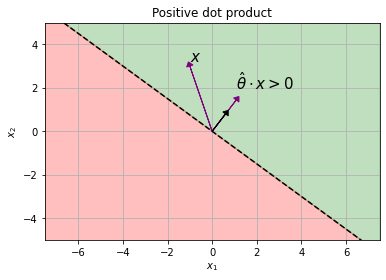
\includegraphics[width=45mm,scale=0.3]{images/classification_images/positive_v_vector_theta_hat.png}
                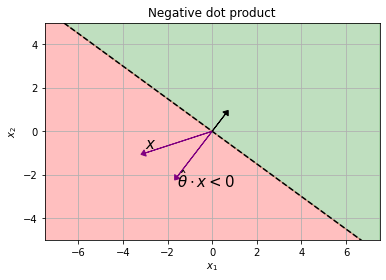
\includegraphics[width=45mm,scale=0.3]{images/classification_images/negative_v_vector_theta_hat.png}
                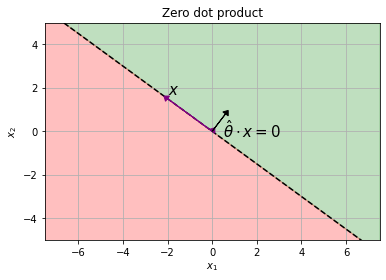
\includegraphics[width=45mm,scale=0.3]{images/classification_images/zero_v_vector_theta_hat.png}
                
                \caption*{Our various dot products can show us where in the space we are.}
        \end{figure}        
        
        So, we can classify things based on the \textbf{sign} of it. Written as an equation, we can define the sign function:\\
        
        \begin{kequation}
            For a \vocab{linear separator} centered on the \purp{origin}, we can do \vocab{binary classification} using the hypothesis
            
            \begin{equation*}
                h(x; \theta) = \text{sign}(\theta \cdot x )= 
                \begin{cases}
                    +1 & \text{if $\theta \cdot x > 0$} \\
                    -1 & \text{otherwise}
                \end{cases}
            \end{equation*}
        \end{kequation}